\title{Layered Architecture}
\author{Brae Webb}
\date{\week{2}}

\maketitle

\section{Introduction}
In the beginning developers created the \textit{big ball of mud}.
It was without form and void, and darkness was over the face of the developers\footnote{Liberties taken from
\href{https://www.biblegateway.com/passage/?search=gen+1\&version=ESV}{Genesis 1:1-2}.}.
The big ball of mud is an architectural style identified by it's lack of architectural style \cite{ballofmud}.
In a big ball of mud architecture, all components of the system are allowed to communicate.
If your GUI code wants to ask the database a question, it will write an SQL query and ask it.
Likewise, if the code which primarily talks to the database decides your GUI needs to be updated a particular way, it will do so.

The ball of mud style is a challenging system to work under.
Modifications can come from any direction at any time.
Akin to a program which primarily uses global variables,
it is hard, if not impossible,
to understand everything that is happening or could happen.

\aside{
Code examples in these notes are works of fiction.
Any resemblance to a working code is pure coincidence.
Having said that, python-esque syntax is often used for it's brevity.
We expect that you can take away the important points from the code examples without getting distracted in the details.
}

\begin{figure}[ht]
\begin{code}[style=python]{}
import gui
import database

button = gui.make_button("Click me to add to counter")
button.onclick(e => 
    database.query("INSERT INTO clicks (time) VALUES {{e.time}}"))
\end{code}
\caption{
A small example of a \textsl{big ball of mud} architecture.
This type of software is fine for experimentation
but not for any code that has to be maintained.
However, it does not work well at scale.
}
\end{figure}

\section{Monolith Architecture}
% Deployment diagram of a monolith.
% Not really necessary, and too painful to fit near page boundaries.
%\begin{wrapfigure}{r}{0.33\textwidth}
%  \begin{center}
%    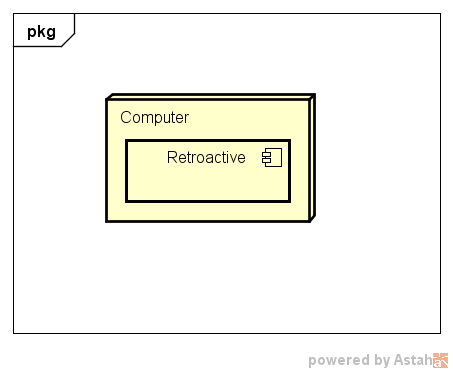
\includegraphics[trim=75 95 98 75,clip,width=0.3\textwidth]{images/monolith_deployed.png}
%  \end{center}
%  \caption{Retroactive Game Deployment Diagram}
%\end{wrapfigure}

\noindent
And architects said, ``let there be structure'', and developers saw that structure was good.
And architects called the structure \emph{modularity}\footnote{Liberties taken from
\href{https://www.biblegateway.com/passage/?search=gen+1\&version=ESV}{Genesis 1:3-5}.}.

The monolithic software architecture is a single deployable application.
There is a single code-base for the application and all developers work within that code-base.
An example monolith application would be one of the games developed by 
\link{DECO2800}{https://my.uq.edu.au/programs-courses/course.html?course_code=DECO2800}
students at \link{UQ}{https://www.uq.edu.au/}.
(e.g. \link{Retroactive}{https://github.com/UQdeco2800/2021-studio-7}).
A monolith should follow design conventions and be well structured and modular
(i.e. it is not a big ball of mud).

Most developers are introduced to the monolith implicitly when they learn to program.
They are told to write a program, and it is a single executable application.
This approach is fine, even preferred, for small projects.
It often becomes a problem for large, complex software systems.

\subsection{Advantages}

The advantages of a monolith are that it is easy to develop, deploy and test.
A single code-base means that all developers know where to find all the source code for the project.
They can use any IDE for development and simple development tools can work with the code-base.
There is no extra overhead that developers need to learn to work on the system.

Being a single executable component, deployment is as simple as copying the executable on to a computer or server.

System and integration testing tends to be easier with a monolith, as end-to-end tests are executing on a single application.
This often leads to easier debugging once errors are found in the software.
All dependencies and logic are within the application.

There are also fewer issues to do with logging, exception handling, monitoring, and even scalability if it is running on a server.

\subsection{Disadvantages}

The drawbacks of a monolith are complexity, coupling and scalability.
Being a single application, as it gets larger and more complex, there is more to understand.
It becomes harder to know how to change existing functionality or add new functionality without creating unexpected side effects.
A catch phrase in software design and architecture is to build complex systems, but not complicated systems.
Monoliths usually become complicated as they grow to deliver complex behaviour.

Related to complexity is coupling, with all behaviour implemented in one system
there tends to be greater dependency between different parts of the system.
The more dependencies that exist, the more difficult it is to understand any one part of the system.
This means it is more difficult to make changes to the system or to identify the cause of defects in the system.

A monolith running on a server can be scaled by running it on multiple servers.
Because it is a monolith, without dependencies on other systems, it is easy to scale and replicate the system.
The drawback is that you have to replicate the entire system on another server.
You cannot scale components of the system independently of each other.
If the persistence logic is creating a bottleneck, you have to copy the entire application on to another server to scale the application.
You cannot user servers that are optimised to perform specialised tasks.

\section{Layered Architecture}

And architects said, ``let there be an API between the components,
and let it separate component from component\footnote{Liberties taken from
\href{https://www.biblegateway.com/passage/?search=gen+1\&version=ESV}{Genesis 1:6-8}.}''.

The first architectural style we will investigate is a layered architecture.
Layered architecture (also called multi-tier or tiered architecture) 
partitions software into specialised components and restricts how those components can communicate with each other.
A layered architecture creates superficial boundaries between the software components, or layers.
Often component boundaries aren't enforced by the technology but by architectural policy.

The creation of these boundaries provides the beginnings of some control over what your software is allowed to do.
Communication between the component boundaries is done via well-specified \textsl{contracts}.
The use of contracts results in each layer knowing precisely how it can be interacted with.
Furthermore, when a layer needs to be replaced or rewritten, it can be safely substituted with a layer fulfilling the contract.

% The isolated components of a layered architecture are normally technically partitioned rather than domain partitioned.

\subsection{Standard Form}

\begin{figure}[ht]
\centering
\begin{tikzpicture}[component/.style={draw, anchor=center, text width=120pt}]
    \node [component](P) at (0,0)  {Presentation Layer};
    \node [component] at (0,-1)  {Business Layer};
    \node [component] at (0,-2)  {Persistence Layer};
    \node [component](D) at (0,-3)  {Database Layer};

    \node[draw, fit=(P) (D)](hardware) {};
\end{tikzpicture}
\caption{The traditional specialised components of a layered architecture.}
\label{fig:traditional-layered}
\end{figure}

The traditional components of a layered architecture are seen in Figure \ref{fig:traditional-layered}.
This style of layered architecture is the four-tier architecture.
Here, our system is composed of a presentation layer, business layer, persistence layer, and database layer.

The presentation layer takes data and formats it in a way that is sensible for humans.
For command line applications, the presentation layer would accept user input and print formatted messages for the user.
For traditional GUI applications, the presentation layer would use a GUI library to communicate with the user.

The business layer is the logic central to the application.
The interface to the business layer is events or queries triggered by the presentation layer.
It's the responsibility of the business layer to determine the data updates or queries required to fulfil the event or query.

The persistence layer is essentially a wrapper over the database,
allowing more abstract data updates or queries to be made by the business layer.
One advantage of the persistence layer is it enables the database to be swapped out easily.

Finally, the database layer is normally a commercial database application like MySQL, Postgres, etc.
which is populated with data specific to the software.
Figure \ref{fig:standard-form-example} is an over-engineered example of a layered architecture.

\begin{figure}[H]
\begin{code}[style=python]{presentation.code}
import gui
import business

button = gui.make_button("Click me to add to counter")
button.onclick(business.click)
\end{code}
\caption{An unnecessarily complicated example of software components separated into the standard layered form.}
\label{fig:standard-form-example}
\end{figure}

\begin{figure}[H]
\ContinuedFloat
\begin{code}[style=python]{business.code}
import persistence

def click():
    persistence.click_counts.add(1)
\end{code}

\begin{code}[style=python]{persistence.code}
import db

class ClickCounter:
    clicks = 0

    def constructor():
        clicks = db.query("SELECT COUNT(*) FROM clicks")

    def get_click():
        return clicks

    def add(amount):
        db.query("INSERT INTO clicks (time) VALUES {{time.now}}")

click_counts = ClickCounter()
\end{code}
\caption{An unnecessarily complicated example of software components separated into the standard layered form.}
\end{figure}

One of the key benefits afforded by a well designed layered architecture is each layer should be interchangeable.
A typical example is an application which starts as a command line application
but can later be adapted to a GUI application by just replacing the presentation layer.

\subsection{Deployment Variations}

While the layered architecture is popular with software deployed on one machine (a non-distributed system),
layered architectures are also often deployed to separate machines.

Each layer can be deployed as separate binaries on separate machines.
A simple, common variant of distributed deployment is separating the database layer,
as shown in figure \ref{fig:layered-db-separated}.
Since databases have well defined contracts and are language independent,
the database layer is a natural first choice for physical separation.

\begin{figure}[ht]
    \centering
    \begin{tikzpicture}[component/.style={draw, anchor=center, text width=120pt}]
        \node [component](P) at (0,0)  {Presentation Layer};
        \node [component](B) at (0,-1)  {Business Layer};
        \node [component](Pe) at (0,-2)  {Persistence Layer};
        \node [component](D) at (0,-3.5)  {Database Layer};
    
        \node[draw, fit=(P) (Pe)](hardware1) {};
        \node[draw, fit=(D)](hardware2) {};

        \draw (hardware1) -- (hardware2);
    \end{tikzpicture}
    \caption{Traditional layered architecture with a separately deployed database.}
    \label{fig:layered-db-separated}
\end{figure}

\pagebreak
In a well designed system, any layer of the system could be physically separated with minimal difficulty.
The presentation layer is another common target, as shown in figure \ref{fig:layered-db-pres-separated}.
Physically separating the presentation layer gives users the ability to only install the presentation layer and allow communication to
other software components to occur via network communication.

\begin{figure}[ht]
    \centering
    \begin{tikzpicture}[component/.style={draw, anchor=center, text width=120pt}]
        \node [component](P) at (0,0)  {Presentation Layer};
        \node [component](B) at (0,-1.5)  {Business Layer};
        \node [component](Pe) at (0,-2.5)  {Persistence Layer};
        \node [component](D) at (0,-4)  {Database Layer};
    
        \node[draw, fit=(P)](hardware1) {};
        \node[draw, fit=(B) (Pe)](hardware2) {};
        \node[draw, fit=(D)](hardware3) {};

        \draw (hardware1) -- (hardware2);
        \draw (hardware2) -- (hardware3);
    \end{tikzpicture}
    \caption{Traditional layered architecture with a separately deployed database and presentation layer.}
    \label{fig:layered-db-pres-separated}
\end{figure}

This deployment form is very typical of web applications.
The presentation layer is deployed as a \mbox{HTML/}JavaScript application which makes network requests to the remote business layer.
The business layer then validates requests and makes any appropriate data updates.

Some database driven appliation generators will separate embedded the application logic in the database code
so that all logic runs on the database server.
The presentation layer is then separated from the application logic,
as shown in figure \ref{fig:layered-pres-separated}.

\begin{figure}[ht]
    \centering
    \begin{tikzpicture}[component/.style={draw, anchor=center, text width=120pt}]
        \node [component](P) at (0,0)  {Presentation Layer};
        \node [component](B) at (0,-1.5)  {Business Layer};
        \node [component](Pe) at (0,-2.5)  {Persistence Layer};
        \node [component](D) at (0,-3.5)  {Database Layer};
    
        \node[draw, fit=(P)](hardware1) {};
        \node[draw, fit=(B) (D)](hardware2) {};

        \draw (hardware1) -- (hardware2);
    \end{tikzpicture}
    \caption{Traditional layered architecture with a separately deployed presentation layer.}
    \label{fig:layered-pres-separated}
\end{figure}

An uncommon deployment variation (figure \ref{fig:uncommon-diagram}) separates
the presentation and business layers from the persistence and database layers.
An updated version of our running example is given in figure~\ref{fig:uncommon-code},
the presentation layer remains the same but the communication between the
business and persistence layers is now via REST.\footnote{\url{https://restfulapi.net/}}

\begin{figure}[ht]
    \centering
    \begin{tikzpicture}[component/.style={draw, anchor=center, text width=220pt}]
        \node [component](P) at (0,0)  {Presentation Layer\hfill \color{gray}192.168.0.20};
        \node [component](B) at (0,-1)  {Business Layer\hfill \color{gray}192.168.0.20};
        \node [component](Pe) at (0,-2.5)  {Persistence Layer\hfill \color{gray}192.168.0.40};
        \node [component](D) at (0,-3.5)  {Database Layer\hfill \color{gray}192.168.0.40};
    
        \node[draw, fit=(P) (B)](hardware1) {};
        \node[draw, fit=(Pe) (D)](hardware2) {};

        \draw (hardware1) -- (hardware2);
    \end{tikzpicture}
    \caption{A contrived example of a deployment variation.}
    \label{fig:uncommon-diagram}
\end{figure}

\begin{figure}[H]
\begin{code}[style=python]{business.code}
import http

def click():
    http.post(
        address="192.168.0.40",
        endpoint="/click/add",
        payload=1
    )
\end{code}

\begin{code}[style=python]{persistence.code}
import db
import http

class ClickCounter:
    ... # as above

click_counts = ClickCounter()

http.on(
    method="post",
    endpoint="/click/add",
    action=(payload => click_counts.add(payload))
)
\end{code}
\caption{Code adapted for the contrived example of a deployment variation.}
\label{fig:uncommon-code}
\end{figure}

\subsection{Closed/Open Layers}

Separating software into layers helps to increase the modularity and isolation of distinct components.
But, of course, components must communicate via their specified contracts, otherwise they wouldn't be particularly useful.
Flows of communication between components are categorized as either \textsl{open} or \textsl{closed}.
A layer, by default, is considered \textsl{closed}.
Closed layers prevent the direct communication between their adjacent layers.
Figure \ref{fig:closed-layers} shows the communication channels (as arrows) in a completely closed architecture.

\begin{figure}[ht]
    \centering
    \begin{tikzpicture}[component/.style={draw, anchor=center, text width=220pt}]
        \node [component](P) at (0,0)  {Presentation Layer\hfill \color{gray}Closed};
        \node [component](B) at (0,-1)  {Business Layer\hfill \color{gray}Closed};
        \node [component](Pe) at (0,-2)  {Persistence Layer\hfill \color{gray}Closed};
        \node [component](D) at (0,-3)  {Database Layer\hfill \color{gray}Closed};
    
        \node[draw, fit=(P) (D)](hardware) {};

        \draw[-Latex] (P) -- (B);
        \draw[-Latex] (B) -- (Pe);
        \draw[-Latex] (Pe) -- (D);
    \end{tikzpicture}
    \caption{All layers closed requiring communication to pass through every layer.}
    \label{fig:closed-layers}
\end{figure}

An architecture where all layers are closed enables maximum isolation.
A change to the communication contracts of any layer will require changes to at most one other layer.
However, there are a number of situations where an \textsl{open} layer can be useful.
Open layers do not require communication to pass through, communication can occur `around' the layer.

\todo{
Thinking about it, I'm not sure that open and closed layers is worth teaching.
I think variations in the physical structures of layers which enables sidecars, etc from Bass would be better.
It's more flexible and enables more obvious examples, i.e. a logging service sidecar
}

\begin{figure}[ht]
    \centering
    \begin{tikzpicture}[component/.style={draw, anchor=center, text width=220pt}]
        \node [component](P) at (0,0)  {Presentation Layer\hfill \color{gray}Closed};
        \node [component](B) at (0,-1)  {Business Layer\hfill \color{gray}Open};
        \node [component](Pe) at (0,-2)  {Persistence Layer\hfill \color{gray}Open};
        \node [component](D) at (0,-3)  {Database Layer\hfill \color{gray}Closed};
    
        \node[draw, fit=(P) (D)](hardware) {};

        \draw[-Latex] (P) -- (B);
        \draw[-Latex] (B) -- (Pe);
        \draw[-Latex] (Pe) -- (D);

        \draw[-Latex] ([xshift=10pt]P.south) -- ([xshift=10pt]Pe.north);
        \draw[-Latex] ([xshift=30pt]P.south) -- ([xshift=30pt]D.north);
        \draw[-Latex] ([xshift=20pt]B.south) -- ([xshift=20pt]D.north);
    \end{tikzpicture}
    \caption{A wolf in layer's clothing \cite{bass2013software}}
    \label{fig:wolf}
\end{figure}

\begin{figure}[ht]
    \centering
    \begin{tikzpicture}[component/.style={draw, anchor=east, fill=gray!40}]
        \node [component, text width=100pt](P) at (0,0)  {Presentation Layer};
        \node [component, text width=120pt](B) at (0,-1)  {Business Layer};
        \node [component, text width=140pt](Pe) at (0,-2)  {Persistence Layer};
        \node [component, text width=160pt](D) at (0,-3)  {Database Layer};

        \def\stairs{([xshift=-10pt]P.north west)
                --([xshift=-10pt,yshift=-9pt]P.west)
                --([xshift=-10pt,yshift=9pt]B.north west)
                --([xshift=-10pt,yshift=-9pt]B.west)
                --([xshift=-10pt,yshift=9pt]Pe.north west)
                --([xshift=-10pt,yshift=-9pt]Pe.west)
                --([xshift=-10pt,yshift=9pt]D.north west)
                --([xshift=-10pt,yshift=-10pt]D.west)
                --([xshift=-40pt]D.south west)}
        \draw \stairs;
    
        \begin{scope}[on background layer]
            \fill[gray!40] \stairs |- cycle;
        \end{scope}
    
        % \node[draw, fit=(P) (D)](hardware) {};
    \end{tikzpicture}
    \caption{A more complicated layered architecture \cite{bass2013software} \todo{Figure is an example of a variation on open/closed layer model (fig 13.2 in bass - reconstruction in progress)}}
    \label{fig:complicated-layers}
\end{figure}

